%!TEX root = ../../../../memoria.tex
\section{Localización}

El inglés no solo ostenta el primer lugar como el idioma más utilizado, \rankingCPT que considera además del porcentaje de población, la distribución geográfica, sino que además es el idioma más usado en los \websitesINT alcanzando la cifra de 59,4\%, seguido tímidamente por Rusia con un 5,9\% \cite{online_world_wide_languages}. Mirando estas cifras se podría concluir que la inclusión de múltiples idiomas en un \siteINT \ecommerceCOM	no reprensentaría ingresos importantes.
El potencial económico \online es de \$45 trillones, de acuerdo a un estudio realizado por \commonSenseAdvisoryNAME \cite{online_world_global_oportunity_multi_languages}.  Sin una sólida estrategia de localización que considere \websitesINT \ecommerceCOM con \textit{multi-idiomas}, será  un desafío tener al alcance de la mano ese \revenueCOM. De hecho, el mismo estudio vislumbró que si solo se tiene una versión en inglés del \siteINT, se estará limitado solo a una tercera parte del total.

%Grow revenue with website localization
%The economic potential of online communication is $45 trillion, according to a recent study by Common Sense Advisory. How exciting! The sky is the limit for your global business.
%Or is it?
%Without a solid localization strategy that incorporates an e-commerce website in multiple languages, it will be a challenge to get within arm’s reach of this revenue. In fact, the same study found that if you have just an English version of your website, you’re limited to only one third of the pot.

¿Cuántos serán los idiomas necesarios para permanecer competitivo en el mundo \online?. Los investigadores dicen que un mínimo de 14. Las marcar mundiales que aspiran a un 95\% de las billeteras \online necesitan de 20 idiomas. Si bien es cierto no es siempre posible mantener contenido \online en 20 idiomas, es difícil negar los beneficios de la localización para regiones específicas alrededor del mundo \cite{online_world_global_oportunity_multi_languages}. Estas son las razones de por qué se considera muy importante la localización en el \frameworkPC y de por qué se aborda esta característica desde los inicios.

Actualmente la aplicación cuenta con un sistema robusto para la localización, permitiendo nuevos idiomas simplemente agregando un archivo \jsonNAME (\refFigura{figure:features:languages_available}).
%How many languages does it take for global businesses to stay competitive online? The research says a minimum of 14. Global brands wanting to appeal to 95 percent of the world’s online wallet need 20 languages. While it isn’t always feasible for a business to translate online content into 20 languages, it’s hard to deny the benefits of website localization for targeted regions around the world.
%Many businesses recognize this and plan to add even more languages to their localization strategy in the future. One example is European-based clothing seller ASOS. They launched a website for the Chinese and Russian markets in 2013 to expand their global footprint. They already had a presence in the United Kingdom, United States, France, Germany and Australia. They saw international sales overall increase by 39 percent with their past website localization initiatives—so they knew that additional language sites would help grow revenue.
%If you’re ready to get a bigger piece of the global e-commerce pie, like ASOS, consider upping the number of languages on your website. Check out the article, Global e-commerce: Are these 5 items in your localization shopping cart?, for tips on how to approach e-commerce website localization.


\begin{figure}[H]
	\centering
	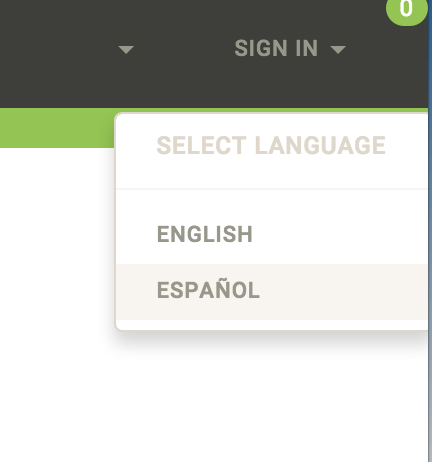
\includegraphics[width=0.3\textwidth]{figuras/languages_available.png}

	\caption{Selección de idioma para el \websiteINT.}
	\label{figure:features:languages_available}
\end{figure}